\chapter{desarrollo y despliegue}
\section{Enfoque metodológico}

El proyecto se estructuró de modo clásico \gls{sdlc} con las siguientes fases:

\begin{enumerate}
    \item Ideación: del concepto y problema general a resolver.
    \item Especificación de requerimientos: Definicion de los requerimientos funcionales y no funcionales, junto con los criterios de aceptación.
    \item Diseño de la solución: Definición de la arquitectura, de los componentes logicos, del modelo de datos y de la experiencia de usuario (mediante maquetas).
    \item Desarrollo y pruebas: Fase de codificación y verificación de que el código cumple con los requerimientos y alcanza satisfactoriamente los criterios de aceptación.
    \item Despliegue a producción y lanzamiento: Fase de despliegue en el entorno productivo y tareas de capacitación y entrenamiento de usuarios (y de equipo de soporte/operaciones)
    \item Operación: fase en la que ya estando el sistema productivo, se le da soporte a los usuarios frente a incidentes.
    \item Decomisado: fase en la que se planifica y ejecuta el decomisado de la aplicación una vez que ya ha cumplido su ciclo de vida (todavía no ha ocurrido esto, ni se espera que ocurra en los proximos 2-3 años)
\end{enumerate}

%Cada fase estando muy bien definida con documentación formal como parte de los entregables de cada fase.

Inicialmente se decidió trabajar con una metodología \emph{Waterfall}, para poder enfocarse en un primer entregable, que pudiera cumplir con la funcionalidad básica de los casos de uso.


Para encarar el desarrollo, también se ensambló un equipo compuesto por los siguientes roles:

\begin{enumerate}
    \item Product Owner: Persona encargada de definir el producto, su roadmap, prioridades y fases de entregas para maximizar el valor de cada entrega, en múltiples fases de desarrollo.
    \item Project Manager: Persona encargada de armar el plan de trabajo con el product owner, los equipos de desarrollo, pruebas, operaciones y entrenamiento, para poder planificar las entregas y luego hacer la coordinar la ejecución y su seguimiento.
    \item Equipo de desarrollo: Equipo responsable por escribir el código y realizar pruebas unitarias y verificaciones iniciales del código. Conformado por programadores especializados en visualización, en logica de negocio y bases de datos. También hubo apoyo part time de un arquitecto para poder trabajar las definiciones estructurales y detalles de arquitectura definidas en la sección anterior.
    \item Equipo de testing: conformado por un líder de testing encargado de desarrollar los planes de pruebas, y desarrollar los casos de pruebas en funcion de las especificaciones de los casos de uso. Testers, encargados de ejecutar los casos de prueba, de distintos tipos, desde pruebas de integración, como así también de regresión y de performance.
    \item Equipo de operaciones: Este equipo es el responsable de operar el sistema una vez desplegado en producción y a la vez de dar continuidad a la operación, en caso de que alguno de los componentes falle por algún problema. Frente alguna situación de falla o reportes de errores de usuario, son la primer capa de atención al usuario y que permite analizar el síntoma y hacer un diagnóstico, para saber si lo reportado por los usuarios es realmente un error del sistema, un problema de experiencia de usuario o de entrenamiento.
    \item Equipo de capacitación: Equipo responsable de generar el material didáctico y planificar junto con el PM las capacitaciones de los usuarios, para poder garantizar una adopción adecuada del producto. También se explica el esquema de soporte en caso de necesitar reportar incidentes.
\end{enumerate}

\newpage
El esquema de trabajo en función de responsabilidades puede resumirse en la siguiente matriz \gls{raci}


\begin{figure}
\begin{tabular}{lcccccc}
\toprule
\textbf{Rol / Fase} & \textbf{Ideación} & \textbf{Reqs} & \textbf{Diseño} & \textbf{Desarrollo } & \textbf{Despliegue} & \textbf{Operación} \\
\midrule
PO & \textbf{A / R} & \textbf{A / R} & C & C & C & I \\
PM & C & C & \textbf{R} & A & \textbf{A / R} & I \\
Architect & C & C & \textbf{A} & R & C & I \\
Desarrollo & I & C & R / C & \textbf{R} & C & I \\
Testing & I & C & C & \textbf{R / C} & C & I \\
Operaciones & I & I & C & I & \textbf{I} & \textbf{R / A} \\
Capacitación & I & A & I & I & \textbf{R} & C \\
\bottomrule
\end{tabular}
    \caption{Matriz \gls{raci}-\gls{sdlc} para el equipo definido}
    \label{fig:raci_matrix} 
\end{figure}

    \newpage

\begin{figure}
\begin{tikzpicture}[
  role/.style={rectangle, draw, rounded corners, align=center, minimum height=1.5cm},
  arr/.style={-{Stealth}, thick}
  ]

  % Nodos
  \coordinate (anchoro) at (-5cm,0cm);
  \node[role, right=10cm of anchoro] (PO) {Product Owner};
  \node[role, below=of PO] (PM) {Project Manager};
  \node[role, below=of PM] (DEV) {Equipo de Desarrollo};
  \node[role, right=of DEV] (TEST) {Equipo de Testing};
  \node[role, below=of TEST] (OPS) {Equipo de Operaciones};
  \node[role, right=of TEST] (TRAIN) {Equipo de Capacitación};

  % Flechas principales
  \draw[arr] (PO) -- (PM);
  \draw[arr] (PM) -- (DEV);
  \draw[arr] (PM) -- (TEST);
  \draw[arr] (PM) -- (OPS);
  \draw[arr] (PM) -- (TRAIN);

  % Interacciones entre equipos
  \draw[arr] (DEV) -- (TEST);
  \draw[arr] (TEST) -- (DEV);
  \draw[arr] (DEV) -- (OPS);
  \draw[arr] (OPS) -- (DEV);

  \draw[arr] (TRAIN) -- (DEV);
  \draw[arr] (TRAIN) -- (OPS);
  \draw[arr] (TRAIN) -- (PM);

\end{tikzpicture}
    \caption{Interacciones entre roles/sub-equipos}
    \label{fig:ways_of_working} 
\end{figure}


En esta metodología de desarrollo waterfall, se encuentran diferentes entornos de trabajo, dedicados a distintos fines y a la vez, a los que se accede, al cumplir satisfactoriamente diferentes verificaciones del ciclo de desarrollo.

\begin{tabular}{l}
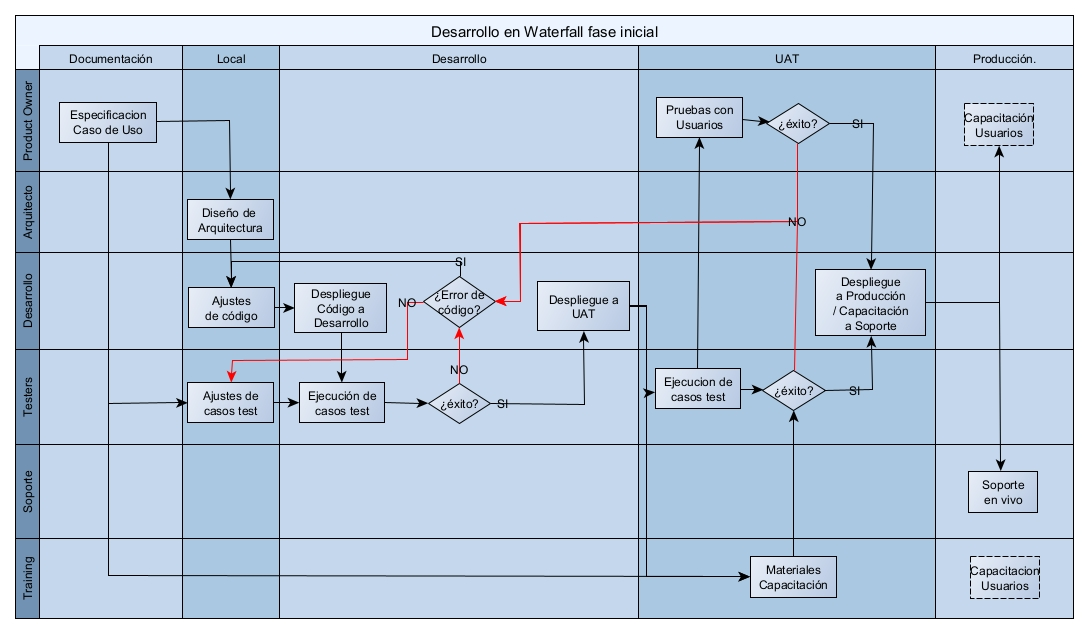
\includegraphics[width=15cm]{waterfal_dev_phase1.jpg}
%\caption{Actividades según roles y entornos}
\end{tabular}

\begin{enumerate}
    \item Entornos locales: En los entornos locales, se trabaja de manera independiente en la documentación de casos de uso, diseño de arquitectura y luego cada desarrollador y tester, trabaja con versiones locales del codigo. En este caso, pueden exisistir múltiples versiones del mismo código que se modifican en paralelo por los distintos desarrolladores, según se hayan dividido las tareas según los skills de los miembros del equipo. (puede ser front end, back end, modelos de datos, apis, etc.).

        A su vez, el equipo de testing, en sus equipos locales, también desarrolla sus casos de prueba, alineados con la funcionalidad definida en la especificación, pero sin interactuar con el equipo de desarrollo, de modo que se toma como base la especifiación y no el código que desarrollan los programadores. De este modo, el equipo de testing se enfoca 100\% en la escencia de la funcionalidad y no necesariamente en cómo se ha desarrollado/implementado la funcionalidad.
    
    
    \item Entorno de Dev: En el entorno de Dev. (o de Desarrollo), es el primero entorno en el que se realizan pruebas del código generado por los multiples desarrolladores, ya combinado en una versión candidata para ser lanzada a producción. Es el espacio donde el equipo de testing puede correr la totalidad de los casos de pruebas que generaron y se evalúan los resultados de las ejecuciones. Si son exitosas, en principio se habilita esa versión de la aplicación/código para ser promovido al entorno de UAT.
    
    En caso de resultar fallidas, el equipo de testing trabaja junto con el equipo de desarrollo para hacer el troubleshooting de aquellos casos fallidos y en función de los hallazgos:
        \begin{enumerate}
            \item se corrije el código porque tenía defectos.
            \item se corrije caso de test porque tenía defectos.
            \item se corrijen el código y el caso de test porque ambos tenían defectos.
        \end{enumerate}
    
    Finalmente, se vuelve a unificar el código y los casos de pruebas ajustados para luego repetir las pruebas en el entorno de desarrollo hasta que todo sea satisfactorio.

    \item Entorno de UAT: Este es el entorno donde el Product Owner, habilita acceso a ciertos usuarios clave, que ayudan a hacer una verificación del sistema para dar el visto bueno para poder pasar el sistema a producción. De surgir fallas, se reportan al equipo de testing y de desarrollo y se realiza el troubleshooting de modo similar al del estadio anterior. De este modo, cualquier falla que se detecta, lleva el proceso al ajuste de código y luego a las pruebas en el estadio anterior.
    
        Una vez que la aplicación se ha desplegado al entorno de UAT, las interfaces de usuario ya son práctiamente definitivas y el equipo de capacitación puede trabajar en el desarrollo de los materiales para la capacitación de los usuarios finales.
    
    \item Entorno de Producción: Una vez que las pruebas en el entorno de UAT han sido superadas con éxito, se hace el pasaje final a producción y ocurren dos actividades escenciales. El product owner queda ya habilitado para comenzar las sesiones de capacitación según el plan de despliegue y entrenamiento y el equipo de desarrollo realiza una transferencia de conocimiento y capacitación (junto con la entrega de la documentación correspondiente) para que el equpo de operaciones, comience a dar el soporte necesario con la plataforma ya en vivo. 
    
    El product owner, junto con el equipo de capacitación (training) hacen el lanzamiento y las campañas de comuniación/entrenamiento con la finalidad de entrenar a los usuarios en el uso del sistema y luego trabajar en la adopción del mismo.
\end{enumerate}

\section{Estrategia de despliegue y fases de rollout.}

Para la estrategia de despliege, se optó, por un enfoque en dos fases. una Fase I, que consistía en un \gls{mvp} con un pequeño grupo piloto de colaboración cercana, de modo de tener un primer acercamiento al uso real del sistema, con quienes se pudo trabajar muy de cerca. Esto permitió que se puedan testear las hipótesis y recolectar feedback valioso, para poder refinar los casos de uso originales.

Luego, se pasó a la fase II, fomentando un crecimiento "orgánico", donde se identificaron equipos clave en el resto de la organización y se fueron sumando gradualmente en un período de 12 meses.

\subsection{Fase I: \gls{mvp} con Grupo piloto}
    
Para hacer el despliegue, se realizó la puesta en producción y se seleccionó un equipo de usuarios que trabajaba con la región de latinoamérica. Ellos tenían muy buena formación técnica y eran los clientes indicados para poder dar el puntapié inicial al despliegue global.

Se trabajó entonces con este equipo en modo piloto inicial y los resultados fueron alentadores. 

Se realizaron las capacitaciones y luego estableció un período de tres meses para dejar rodar la solución y a la vez evaluar la estabilidad, performance y mejorar temas necesarios que no habían sido considerados como para poder luego hacer el rollout global.

\subsection{Fase II: Expansión y escalamiento a más áreas y usuarios}

Ya con el piloto satisfactorio, una lista mínima de mejoras ya implementadas y el equipo redefinido junto con la metodología, se decidió expandir el piloto al resto de las regiones y otros equipos corporativos. El despliege completo duró aproxiamdamente 6 meses más y a medida que se fue avanzando cada vez se fue simplificando más el proceso de "onboarding" de nuevos usuarios.

Se adoptó un enfoque de entrenamiento para los creadores de contenidos y ellos a su vez comenzaron a promocionarlo y entrenar a sus propios usuarios y en muchos casos, cuando había usuarios que ya usaban el portal por otros creadores de contenido, preguntaban proactivamente por qué faltaban agregar más contenidos, con lo cual el crecimiento se dio de modo orgánico y natural.

\section{Plan de comunicación y capacitación}
El plan de comunicación y de capacitación, se diseñó de modo de acompañar las fases de despliegue por grupos de usuarios y audiencias. Se encaró un enfoque de \gls{cop}, que permitió crear un universo de usuarios general, con algunos más "expertos" que ayudaron a disceminar las mejores prácticas. 

se identificaron dichos usuarios líderes o clave y se hizo una capacitación del estilo \gls{ttt}, para poder hacerlo en múltiples olas y a la vez de modo federado y escalable.

Los materiales de soporte y guías de usuario, se defineron en dos niveles: 
\begin{enumerate}
    \item Guía específica para usuarios con privilegios de publicación y administración de contenidos
    \item Guía para usuarios finales, que en realidad estaba integrada al portal, e incluso la misma interfaz era bastante auto descriptiva.
\end{enumerate}

\section{Mecanismos de soporte post-lanzamiento}

Dentro del esquema de soporte, se trabajó con un equipo corporativo que maneja un esquema de soporte de dos niveles. El primer nivel, orientado a preguntas simples y que son de solucion fácil, como pueden ser problemas de conectividad, instrucciones básicas sobre el uso del portal o eventualmente sobre alguno de los reportes. Si el primer nivel, no puede resolver satisfactoriamente la consulta del usuario, entonces se derivaba a un segundo nivel donde se identificaba, según la naturaleza de la consulta, qué acción seguir y qué grupo debía darle seguimiento.

Es importante destacar que el objetivo del equipo de nivel 2, es garantizar la continuidad del servicio y mantener el sistema disponible y los accesos de los usuarios activados.

En caso de que los usuarios finales hayan reportado un comportamiento compatible con un defecto o bug, entonces se derivaba al equipo de desarrollo para seguir con máxima prioridad un proceso de troubleshooting y análisis de causa raíz, para a su vez aplicar una solución definitiva.


\section{Gestión de calidad y ajustes/mejoras metodológicas}


Inicialmente, la calidad del desarrollo se fue monitoreando mediante el equipo de testing. EL leader de testing había creado un plan de pruebas y estas pruebas eran ejecutadas y documentadas rigurosamente antes de realizar pasajes a producción. 


En caso de encontrar errores, se notificaban registraban en una plataforma que utilizabamos para tal fin y se compartían con el equipo de desarrollo y luego de corregirse, se re-verificaban. 


El proceso era muy manual y no permitía, ni gran agilidad, ni múltiples y rápidas iteraciones a la hora de lanzar nuevas versiones a producción.


Después de un período inicial de desarrollo de 6 meses, se logró alcanzar el primer hito, donde se implementaron de manera básica todos los casos de uso definidos inicialmente. 


Esto por un lado permitió ofrecer un MVP útil y funcional y a la vez, detectar oportunidades de mejora y evoluciones posibles, ya con el sistema rodando en el entorno de producción.


Para poder encarar sucesivas iteraciones en la evolución de la plataforma, se tuvo que cambiar drásticamente la composición del equipo, como así también la metodología de desarrollo, de modo tal de poder responder on mayor agilidad a los cambios y necesidades aumentando significativamente calidad y reduciendo los plazos de entrega.


Los cambios, fueron sustantivos y afectaron, no sólo la metodología de desarrollo, sino también la composición del equipo de desarrollo y operaciones.


Las principales causas para revisar la forma de trabajo fueron las siguientes:
El esfuerzo manual de testeo, por parte del equipo de testing era excesivo, lento y un verdadero cuello de botella. La forma en la que se documentaban los defectos, a veces era inconsistente y se podían duplicar y a medida que la complejidad de la aplicación aumentaba, los casos de pruebas y sus tiempos de ejecución crecían de modo exponencial. La complejidad y diversidad casuística aumentaba a un ritmo mucho mayor que el código que la soportaba y era fundamental buscar alternativas.


Esto además tenía un impacto muy negativo en los ciclos de entrega, haciendonos demorar meses hasta que una versión inicial y funcional, llegó a un punto de madurez que la hizo "usable".


Adicionalmente, había problemas en la calidad del código desarrollado por los desarrolladores, porque al demorarse las entregas, la presión por terminar aumentaba e impactaba los entregables generando retrabajo. 


Finalmente, cuando llegaban las versiones al entorno de producción, notamos que en varias ocasiones, a pesar de haber pasado satisfactoriamente las fases de testeo y control de calidad, tenían defectos y el equipo de operaciones, tampoco era efectivo a la hora de resolver algunos incidentes, por falta de conocimiento de la aplicación, y las capacitaciones que el equipo de desarrollo les daba al hacer los despliegues productivos, eran complejas o insuficientes.

\begin{table} 
    \centering
    \begin{tabular}{|c|c|c|c|}\hline
        \textbf{Actividades}&  \textbf{Waterfall}&  \textbf{DevOps Interino}&  \textbf{DevOps Final}\\\hline
         Esquema de entregas&  1 x Trimestre &  1 x Mes & 1-3 x Semana  \\\hline
         Cobertura del código& $\approx 25$\% &  $\approx 25$\%&  $\approx 50$\%\\\hline
         Pruebas de Regresión (hs)&  24&  1&  2\\\hline
         Tiempos de Hand Over (hs)& 8&  4&  -\\\hline
         Tasa de defectos desde Prod\\ (vs trabajo nuevo x mes)&  $\approx 30$\%&  $\approx 15$\%&  $\approx 5$\%\\\hline
    \end{tabular}
    \caption{Mejoras metodológicas}
    \label{tab:water_to_devops_method}
\end{table}

A continuación, se detalla cómo ha evolucionado la composición del equipo, a medida que se avanzó con la transformación metodológica, comparando \gls{fte}.

\begin{table}
    \centering
    \begin{tabular}{|c|c|c|c|}\hline
        \textbf{Composición del Equipo}&  \textbf{Waterfall}&  \textbf{DevOps Interino}&  \textbf{DevOps Final}\\\hline
         ProductOwner&  1 &  1 & 1  \\\hline
         PM/ScrumMaster& 1 &  1&  1\\\hline
         Desarroladores&  4&  4&  4\\\hline
         Arquitecto& 0,3&  0,3&  0,3\\\hline
         DevOps Engineer& 0&  0,1&  0,1\\\hline
         Lead de Test& 1&  1&  0\\\hline
         Testers& 4&  3&  0\\\hline
         Testers+& 0&  2&  2\\\hline
         Training& 0,3&  0,3&  0,3\\\hline
         Support Lead& 1&  0&  0\\\hline
         Support& 1&  0&  0\\\hline
         Total & 13,9&  13,4&  8,4\\\hline         
         Evolucion s\% & 100\%& $\approx 96$ \% &  $\approx 60$\%\\\hline         
        \end{tabular}
    \caption{Evolución del Equipo}
    \label{tab:water_to_devops_team}
\end{table}
